%%%%%%%%%%%%%%%%%%%%%%%%%%%%%%%%%%%%%%%%%
% Beamer Presentation
% LaTeX Template
% Version 1.0 (10/11/12)
%
% This template has been downloaded from:
% http://www.LaTeXTemplates.com
%
% License:
% CC BY-NC-SA 3.0 (http://creativecommons.org/licenses/by-nc-sa/3.0/)
%
%%%%%%%%%%%%%%%%%%%%%%%%%%%%%%%%%%%%%%%%%

%----------------------------------------------------------------------------------------
%	PACKAGES AND THEMES
%----------------------------------------------------------------------------------------

\documentclass{beamer}

\mode<presentation> {

% The Beamer class comes with a number of default slide themes
% which change the colors and layouts of slides. Below this is a list
% of all the themes, uncomment each in turn to see what they look like.

%\usetheme{default} % +
%\usetheme{AnnArbor}
%\usetheme{Antibes}
%\usetheme{Bergen}
%\usetheme{Berkeley} % +
%\usetheme{Berlin}
%\usetheme{Boadilla} % +
%\usetheme{CambridgeUS}
%\usetheme{Copenhagen}
%\usetheme{Darmstadt}
%\usetheme{Dresden} 
%\usetheme{Frankfurt} % +
%\usetheme{Goettingen}
%\usetheme{Hannover}
%\usetheme{Ilmenau}
%\usetheme{JuanLesPins}
%\usetheme{Luebeck}
%\usetheme{Madrid} % +
%\usetheme{Malmoe}
%\usetheme{Marburg}
%\usetheme{Montpellier}
%\usetheme{PaloAlto}
%\usetheme{Pittsburgh}
%\usetheme{Rochester}
\usetheme{Singapore} % +
%\usetheme{Szeged}
%\usetheme{Warsaw}

% As well as themes, the Beamer class has a number of color themes
% for any slide theme. Uncomment each of these in turn to see how it
% changes the colors of your current slide theme.

%\usecolortheme{albatross}
%\usecolortheme{beaver}
%\usecolortheme{beetle}
%\usecolortheme{crane}
%\usecolortheme{dolphin}
%\usecolortheme{dove}
%\usecolortheme{fly}
%\usecolortheme{lily}
%\usecolortheme{orchid}
%\usecolortheme{rose}
%\usecolortheme{seagull}
%\usecolortheme{seahorse}
%\usecolortheme{whale}
%\usecolortheme{wolverine}

%\setbeamertemplate{footline} % To remove the footer line in all slides uncomment this line
%\setbeamertemplate{footline}[page number] % To replace the footer line in all slides with a simple slide count uncomment this line

%\setbeamertemplate{navigation symbols}{} % To remove the navigation symbols from the bottom of all slides uncomment this line
}


%\logo{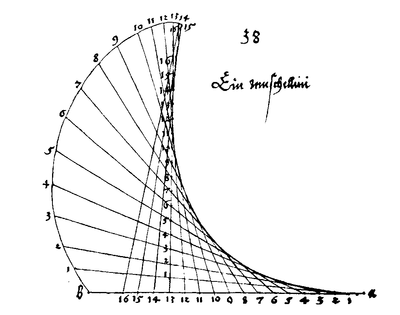
\includegraphics[height=1cm]{./images/logo.png}}


\usepackage{graphicx} % Allows including images
\usepackage{booktabs} % Allows the use of \toprule, \midrule and \bottomrule in tables
\usepackage{caption}
\usepackage{subcaption}
\usepackage{changepage}
\usepackage{color}
%\usepackage{tcolorbox}

%----------------------------------------------------------------------------------------
%	TITLE PAGE
%----------------------------------------------------------------------------------------

\title[Other thing]{Enter Title}

\author{\textcolor{blue}{Marvin Glaser\\}
\vspace{2mm}\footnotesize{Special Thanks: Gabriel Wittum, Arne N\"agel, Tristan Scheidemann, Yannick Rosam, Devansh Rastogi}} % Your name
\institute[G-CSC] % Your institution as it will appear on the bottom of every slide, may be shorthand to save space
{
Goethe Universtiy Frankfurt - Center for Scientific Computing \\ % Your institution for the title page
\medskip
%\textit{john@smith.com} % Your email address
}
%\date{\today} % Date, can be changed to a custom date

\begin{document}

%----------------------------------------------------------------------------------------
%	PRESENTATION SLIDES
%----------------------------------------------------------------------------------------


%\begin{frame}
%	\titlepage % Print the title page as the first slide
%\end{frame}

%----------------------------------------------------------------------------------------
\begin{frame}
\frametitle{Overview} 
\tableofcontents 
\end{frame}

%----------------------------------------------------------------------------------------
%	SECTION FORMATING
%----------------------------------------------------------------------------------------

%\AtBeginSection[]{
%  \begin{frame}
%  \vfill
%  \centering
%  \begin{beamercolorbox}[sep=8pt,center,shadow=true,rounded=true]{title}
%    \usebeamerfont{title}\insertsectionhead\par%
%  \end{beamercolorbox}
%  \vfill
%  \end{frame}
%}

%----------------------------------------------------------------------------------------
%----------------------------------------------------------------------------------------



\section{Model}
\begin{frame}
	\frametitle{Model - Background}
	\begin{enumerate}[$\bullet$]
		\item SEIRD PDE model, based on Arnes/Devanshs "evaluate.lua" \& Tristans ConstrainedOptimization
		\item Solvers used: Gauss-Newton / Particle Swarm Optimization
		\item Loss function $L: (data_{original}(t) - data_{simulated}(t))^2 $
		\item SEIRD classes derived of RKI case numbers\\(01.09.2020 - 15.11.2020)
		\item Grid: 2D of Hessen, 26 discricts, 1075 vertices
		\item In the model $\kappa$ (governs ratio between $E\rightarrow I$ and $E\rightarrow R$ transition) was set to 1
			$\rightarrow$ no transision between E and R
			Reasoning given in summary details at the end
		\item My current interpretation of the results is given in the summary at the end
	\end{enumerate}

\end{frame}

\begin{frame}
	\frametitle{Model - Class definition}
	(\textcolor{red}{E} and \textcolor{red}{I} have changed definition compared to Devanshs thesis)\newline
	\begin{enumerate}[$\bullet$]
		\item (S)usceptibles: Population that has not been in contact with the virus
		\item \textcolor{red}{(E)xposed}: Infected population, has no symptoms yet and is therefor spreading the virus
		\item \textcolor{red}{(I)nfected}: Infected population with symptoms, in isolation or not infectious anymore
		\item (R)ecovered: Infected that have overcome the infection. Cannot spread the virus or get infected again
		\item (D)eceased: Deceased population, does not spread the virus
	\end{enumerate}

\end{frame}
%----------------------------------------------------------------------------------------

\section{Susceptible simulations}
\subsection{Background}
\begin{frame}
	\frametitle{Susceptible simulations- Overview}
	\begin{enumerate}[$\bullet$]
		\item Results below created using a Gauss-Newton solver
		\item 76 datapoints (day 0 - 75) were used for the simulation
		\item Both $\alpha$ (S$\rightarrow$E, infection spreading) and $qq$ (E$\rightarrow$I, time till symptom onset) were optimized in these experiments
		\item Simulations were repeated with 60 and 50 datapoints\\(days 0 - 60/50) to see if the results are similar
	\end{enumerate}
	\vspace{0.5cm}
	Results of variable optimization day 0 - 75:
	\begin{center}
	\begin{tabular}{|c|c|}
		\hline $\alpha$ & 0.197630304390785 \\
		\hline $qq$ & 6.67500068384405 \\ \hline
	\end{tabular}
	\end{center}
\end{frame}

\subsection{Results}
\begin{frame}
	\frametitle{Susceptible simulations - Presentation style}
	\begin{enumerate}[$\bullet$]
		\item x-axis: time t (days) of simulation \newline
			y-axis: sum of all Exposed up to time t
		\item "Sum of newly Exposed till t" is shown insead of "decrease of Susceptibles" for easier readability\\
			(otherwise hard to read, since only a fraction of S is infected)
		\item For presentation, results are grouped into "fitting" (simulation trend matches original data) and "too low/high" trends
		\item "too high" and "too low" show a weaker (upper image) and a more extreme (lower image) example
	\end{enumerate}
\end{frame}

\begin{frame}
	\frametitle{Susceptible simulation, day 0 - 75}
	\begin{center}
		\begin{figure}
			\begin{adjustwidth}{-0.8cm}{}
			\begin{tabular}{c|c|c}
				fitting & too high & too low \\
				\includegraphics[width=0.35\textwidth]{./images/extrapolation75/10_Limburg-Weilburg.pdf}
					& \includegraphics[width=0.35\textwidth]{./images/extrapolation75/19_Frankfurt-am-Main.pdf}
					& \includegraphics[width=0.35\textwidth]{./images/extrapolation75/20_Offenbach-am-Main.pdf} \\
				\includegraphics[width=0.35\textwidth]{./images/extrapolation75/11_Giessen.pdf}
					& \includegraphics[width=0.35\textwidth]{./images/extrapolation75/24_Darmstadt-Dieburg.pdf}
					& \includegraphics[width=0.35\textwidth]{./images/extrapolation75/26_Bergstrasse.pdf}
			\end{tabular}
			\end{adjustwidth}
		\end{figure}
	\end{center}
\end{frame}

\begin{frame}
	\frametitle{Susceptible simulation}
	\textbf{Notes and thoughts:}
	\begin{enumerate}[$\bullet$]
		\item Using the entire dataset (day 0 - 75) for simulation leads to mixed results
		\item To give a "feel" for the entire dataset: I would consider\\
			- 5 regions to have a fitting trend\\
			- 4 regions to have  a trend that is too high\\
			- 17 regions to have a trend that is too low
		\item The slides below show the results of parameter estimation with 60 and 50 days respectively. The same regions as above are shown (for compairibilty)
		\item Data was extrapolated to visualize the trend. This was done using numpy polyfit (Polynomial fit, degree 3)
	\end{enumerate}
\end{frame}

\begin{frame}
	\frametitle{Susceptible trends 60d}
	\begin{center}
		\begin{figure}
			\begin{adjustwidth}{-0.8cm}{}
			\begin{tabular}{ccc}
				prev. fitting & prev. high & prev. low \\
				\includegraphics[width=0.35\textwidth]{./images/extrapolation60/10_Limburg-Weilburg.pdf}
					& \includegraphics[width=0.35\textwidth]{./images/extrapolation60/19_Frankfurt-am-Main.pdf}
					& \includegraphics[width=0.35\textwidth]{./images/extrapolation60/20_Offenbach-am-Main.pdf} \\
				\includegraphics[width=0.35\textwidth]{./images/extrapolation60/11_Giessen.pdf}
					& \includegraphics[width=0.35\textwidth]{./images/extrapolation60/24_Darmstadt-Dieburg.pdf}
					& \includegraphics[width=0.35\textwidth]{./images/extrapolation60/26_Bergstrasse.pdf}
			\end{tabular}
			\end{adjustwidth}
		\end{figure}
	\end{center}
\end{frame}

\begin{frame}
	\frametitle{Susceptible trends 50d}
	\begin{center}
		\begin{figure}
			\begin{adjustwidth}{-0.8cm}{}
			\begin{tabular}{ccc}
				prev. fitting & prev. high & prev. low \\
				\includegraphics[width=0.35\textwidth]{./images/extrapolation50/10_Limburg-Weilburg.pdf}
					& \includegraphics[width=0.35\textwidth]{./images/extrapolation50/19_Frankfurt-am-Main.pdf}
					& \includegraphics[width=0.35\textwidth]{./images/extrapolation50/20_Offenbach-am-Main.pdf} \\
				\includegraphics[width=0.35\textwidth]{./images/extrapolation50/11_Giessen.pdf}
					& \includegraphics[width=0.35\textwidth]{./images/extrapolation50/24_Darmstadt-Dieburg.pdf}
					& \includegraphics[width=0.35\textwidth]{./images/extrapolation50/26_Bergstrasse.pdf}
			\end{tabular}
			\end{adjustwidth}
		\end{figure}
	\end{center}
\end{frame}


%----------------------------------------------------------------------------------------

\section{Sensitivity analysis}
\subsection{Background}
\begin{frame}
	\frametitle{Sensitivity plot $\alpha$ vs. $qq$}
	\begin{enumerate}[$\bullet$]
		\item The folling slides show a sensitivity analysis of $\alpha$ vs $qq$
		\item As above, only the Susceptible group was optimized
		\item 4000 datapoints with randomly chosen $\alpha$ and $qq$ values are scatter plotet against the total loss
		\item x/z - axis: $\alpha$ and $qq$\\
			y - axis: loss ($e^{9}$)
		\item color code: red = high loss, green = low loss
		\item The plots may not show all datapoints, since I set constrains for min/max $\alpha$, $qq$ and loss\\
			This is done to highlight specific areas
	\end{enumerate}
\end{frame}

\subsection{Results}
\begin{frame}
	\frametitle{Sensitivity plot, region overview}
	\begin{center}
		\begin{tabular}{|c|c|c|c|}
			\hline & $alpha$ & $qq$ & loss \\
			\hline range & $0.05-0.35$ & $5.5-8.0$ & $2.5e^{8}-4.5e^{13}$\\
			\hline
		\end{tabular}
		\begin{figure}
			%\begin{adjustwidth}{-1.8cm}{}
			%\begin{tabular}{cc}
				\hspace{-1.3cm}
				\includegraphics[width=0.6\textwidth]{./images/sensitivity/overview/sensitivity0.pdf}\hspace{-1.0cm}% &
				\includegraphics[width=0.6\textwidth]{./images/sensitivity/overview/sensitivity1.pdf}
			%\end{tabular}
			%\end{adjustwidth}
		\end{figure}
		\textcolor{red}{(carefull, $\alpha$ and $qq$ are fipping between these two images)}
	\end{center}
\end{frame}

\begin{frame}
	\frametitle{Sensitivity plot, transition area high/low loss}
	\begin{center}
		\begin{tabular}{|c|c|c|c|}
			\hline & $alpha$ & $qq$ & loss \\
			\hline range & $0.15-0.245$ & $5.5-8.0$ & $2.5^{8}-1.0e^{10}$\\
			\hline
		\end{tabular}

		\begin{figure}[htbp]
			%\begin{adjustwidth}{-2.0cm}{}
			%\begin{tabular}{rl}
				\hspace{-1.4cm}
				\includegraphics[width=0.6\textwidth]{./images/sensitivity/loss9.9e9/sensitivity1.pdf}\hspace{-1.0cm} %&
				\includegraphics[width=0.6\textwidth]{./images/sensitivity/loss9.9e9/sensitivity5.pdf}
			%\end{tabular}
			%\end{adjustwidth}
		\end{figure}
	\end{center}
\end{frame}

\begin{frame}
	\frametitle{Sensitivity plot $\alpha$ vs. $qq$}
	\textbf{Notes and thoughts:}
	\begin{enumerate}[$\bullet$]
		\item The loss function seems sensitivity to both $\alpha$ and $qq$. Generally, a higher $qq$ seems to encurage a higher loss, but this also strongly depends on $\alpha$
		\item There appears to be a "valley", where both $\alpha$ and $qq$ are in an "equilibrium" to minimize the loss
		\item The following slides show the same experimental data, but all datapoints with loss $>$ 2.7e9 are removed. This acts like a "zoom in" on the valley part of the image
	\end{enumerate}
\end{frame}

\begin{frame}
	\frametitle{Sensitivity plot, highlighting optimal $alpha$/$qq$ ratio}
	\begin{center}
		\begin{tabular}{|c|c|c|c|}
			\hline & $alpha$ & $qq$ & loss \\
			\hline range & $0.15-0.24$ & $5.5-8.0$ & $2.5^{8}-2.7e^{9}$\\
			\hline
		\end{tabular}
		\begin{figure}
			%\begin{adjustwidth}{-2.0cm}{}
			%\begin{tabular}{cc}
				\hspace{-1.4cm}
				\includegraphics[width=0.6\textwidth]{./images/sensitivity/loss2.7e9/sensitivity1.pdf}\hspace{-1cm}% &
				\includegraphics[width=0.6\textwidth]{./images/sensitivity/loss2.7e9/sensitivity2.pdf}
			%\end{tabular}
			%\end{adjustwidth}
		\end{figure}
		%\includegraphics[width=0.7\textwidth]{./images/}
	\end{center}
\end{frame}




%----------------------------------------------------------------------------------------

\section{Summary}
\subsection{Current state}
\begin{frame}
	\frametitle{Current state - Software}
	\begin{enumerate}[$\bullet$]
		\item The model itself is in a working state and can reliably produce a somewhat accurate trends on a 76 day timescale
		\item Given some code adjustments, the time frame can be shifted to simulate a different data set (same region)
		\item 2D-grids can be changed pretty easy, if a new grid is provided
		\item While the Gauss-Newton solver works well for optimizing $\alpha$ and $qq$ on the Susceptible dataset, it has issues on others\\
			Particle Swarm Optimization) can be used instead, but this is much more time consuming
	\end{enumerate}
\end{frame}

\begin{frame}
	\frametitle{Current state - Model}
	\begin{enumerate}[$\bullet$]
		\item The biggest current modelling issue is the strong difference between different regions\\
			Reason is probably a lack of factors, that adjust the variables (e.g. an adjustment of $\alpha$ based population density)
		\item Another factor could be the loss calculation method. Loss calculation based on the squared differnce between sim.
			and real data, seems to bias towards high population regions (due to greater numbers)
		\item Changing the definition of exposed and infected was an attempt to better model intitial process of infection (spreading the virus mainly
			before symptom onset), but made it very difficult to find/approximate real world data for $E\rightarrow R$ transition
	\end{enumerate}
\end{frame}

\subsection{Questions}

\begin{frame}
	\frametitle{Questions}
	\begin{enumerate}[$\bullet$]
		\item Teser
	\end{enumerate}

\end{frame}
%\section{Appendix}
%\subsection{Details}
%\begin{frame}
%	\frametitle{Details}
%	\begin{enumerate}[$\bullet$]
%		\item res1
%	\end{enumerate}
%
%\end{frame}

%\subsection{Data}
%\begin{frame}
%	\frametitle{Sensitivity plot, all datapoints shown}
%	\begin{center}
%		\includegraphics[width=0.95\textwidth]{./images/sensitivity/loss9.9e9/sensitivity0.pdf}
%	\end{center}
%\end{frame}
%
%\begin{frame}
%	\frametitle{Sensitivity plot, all datapoints shown}
%	\begin{center}
%		\includegraphics[width=0.95\textwidth]{./images/sensitivity/loss9.9e9/sensitivity1.pdf}
%	\end{center}
%\end{frame}
%\begin{frame}
%	\frametitle{Sensitivity plot, all datapoints shown}
%	\begin{center}
%		\includegraphics[width=0.95\textwidth]{./images/sensitivity/loss9.9e9/sensitivity2.pdf}
%	\end{center}
%\end{frame}
%
%\begin{frame}
%	\frametitle{Sensitivity plot, all datapoints shown}
%	\begin{center}
%		\includegraphics[width=0.95\textwidth]{./images/sensitivity/loss9.9e9/sensitivity3.pdf}
%	\end{center}
%\end{frame}
%\begin{frame}
%	\frametitle{Sensitivity plot, all datapoints shown}
%	\begin{center}
%		\includegraphics[width=0.95\textwidth]{./images/sensitivity/loss9.9e9/sensitivity4.pdf}
%	\end{center}
%\end{frame}
%
%\begin{frame}
%	\frametitle{Sensitivity plot, all datapoints shown}
%	\begin{center}
%		\includegraphics[width=0.95\textwidth]{./images/sensitivity/loss9.9e9/sensitivity5.pdf}
%	\end{center}
%\end{frame}
%
%
%\begin{frame}
%	\frametitle{Sensitivity plot, loss caped at 2.7e9 ("zoom in")}
%	\begin{center}
%		\includegraphics[width=0.95\textwidth]{./images/sensitivity/loss2.7e9/sensitivity0.pdf}
%	\end{center}
%\end{frame}
%
%\begin{frame}
%	\frametitle{Sensitivity plot, loss caped at 2.7e9 ("zoom in")}
%	\begin{center}
%		\includegraphics[width=0.95\textwidth]{./images/sensitivity/loss2.7e9/sensitivity1.pdf}
%	\end{center}
%\end{frame}
%\begin{frame}
%	\frametitle{Sensitivity plot, loss caped at 2.7e9 ("zoom in")}
%	\begin{center}
%		\includegraphics[width=0.95\textwidth]{./images/sensitivity/loss2.7e9/sensitivity2.pdf}
%	\end{center}
%\end{frame}
%
%\begin{frame}
%	\frametitle{Sensitivity plot, loss caped at 2.7e9 ("zoom in")}
%	\begin{center}
%		\includegraphics[width=0.95\textwidth]{./images/sensitivity/loss2.7e9/sensitivity3.pdf}
%	\end{center}
%\end{frame}
%\begin{frame}
%	\frametitle{Sensitivity plot, loss caped at 2.7e9 ("zoom in")}
%	\begin{center}
%		\includegraphics[width=0.95\textwidth]{./images/sensitivity/loss2.7e9/sensitivity4.pdf}
%	\end{center}
%\end{frame}
%
%\begin{frame}
%	\frametitle{Sensitivity plot, loss caped at 2.7e9 ("zoom in")}
%	\begin{center}
%		\includegraphics[width=0.95\textwidth]{./images/sensitivity/loss2.7e9/sensitivity5.pdf}
%	\end{center}
%\end{frame}



%----------------------------------------------------------------------------------------
%\begin{frame}
%	\frametitle{Sensitivity plot $\alpha$ vs. $qq$}
%	\begin{center}
%		\begin{figure}
%			\begin{adjustwidth}{-0.8cm}{}
%			\begin{tabular}{ccc}
%				\includegraphics[width=0.35\textwidth]{./images/sensitivity/loss9.9e9/sensitivity0.pdf}
%					& \includegraphics[width=0.35\textwidth]{./images/sensitivity/loss9.9e9/sensitivity1.pdf}
%					& \includegraphics[width=0.35\textwidth]{./images/sensitivity/loss9.9e9/sensitivity2.pdf} \\\hline
%				\includegraphics[width=0.35\textwidth]{./images/sensitivity/loss9.9e9/sensitivity3.pdf}
%					& \includegraphics[width=0.35\textwidth]{./images/sensitivity/loss9.9e9/sensitivity4.pdf}
%					& \includegraphics[width=0.35\textwidth]{./images/sensitivity/loss9.9e9/sensitivity5.pdf}
%			\end{tabular}
%			\end{adjustwidth}
%		\end{figure}
%		%\includegraphics[width=0.7\textwidth]{./images/}
%	\end{center}
%\end{frame}
%\begin{frame}
%	\frametitle{Sensitivity plot $\alpha$ vs. $qq$}
%	\begin{center}
%		\begin{figure}
%			\begin{adjustwidth}{-0.8cm}{}
%			\begin{tabular}{ccc}
%				\includegraphics[width=0.35\textwidth]{./images/sensitivity/loss2.7e9/sensitivity0.pdf}
%					& \includegraphics[width=0.35\textwidth]{./images/sensitivity/loss2.7e9/sensitivity1.pdf}
%					& \includegraphics[width=0.35\textwidth]{./images/sensitivity/loss2.7e9/sensitivity2.pdf} \\\hline
%				\includegraphics[width=0.35\textwidth]{./images/sensitivity/loss2.7e9/sensitivity3.pdf}
%					& \includegraphics[width=0.35\textwidth]{./images/sensitivity/loss2.7e9/sensitivity4.pdf}
%					& \includegraphics[width=0.35\textwidth]{./images/sensitivity/loss2.7e9/sensitivity5.pdf}
%			\end{tabular}
%			\end{adjustwidth}
%		\end{figure}
%		%\includegraphics[width=0.7\textwidth]{./images/}
%	\end{center}
%\end{frame}
%----------------------------------------------------------------------------------------


%----------------------------------------------------------------------------------------


\end{document} 
